%%%%%%%%%%%%%%%%%%%%%%%%%%%%%%%%%%%%%%%%%%%%%%%%%%%%%%%%%%%%%%%%%%%%%%%%%%%%%%%%
%%%%%%%%%%%%%%%%%%%%%%%%%%%%%%%%%%%%%%%%%%%%%%%%%%%%%%%%%%%%%%%%%%%%%%%%%%%%%%%%
%%                                                                            %%
%% thesistemplate.tex version 3.10 (2018/04/24)                               %%
%% The LaTeX template file to be used with the aaltothesis.sty (version 3.10) %%
%% style file.                                                                %%
%% This package requires pdfx.sty v. 1.5.84 (2017/05/18) or newer.            %%
%%                                                                            %%
%% This is licensed under the terms of the MIT license below.                 %%
%%                                                                            %%
%% Copyright 2017-2018, by Luis R.J. Costa, luis.costa@aalto.fi,              %%
%% Copyright 2017-2018 documentation in Finnish in the template by Perttu     %%
%% Puska, perttu.puska@aalto.fi                                               %%
%% Copyright Swedish translations 2017-2018 by Elisabeth Nyberg,              %%
%% elisabeth.nyberg@aalto.fi and Henrik Wallén, henrik.wallen@aalto.fi        %%
%%                                                                            %%
%% Permission is hereby granted, free of charge, to any person obtaining a    %%
%% copy of this software and associated documentation files (the "Software"), %%
%% to deal in the Software without restriction, including without limitation  %%
%% the rights to use, copy, modify, merge, publish, distribute, sublicense,   %%
%% and/or sell copies of the Software, and to permit persons to whom the      %%
%% Software is furnished to do so, subject to the following conditions:       %%
%% The above copyright notice and this permission notice shall be included in %%
%% all copies or substantial portions of the Software.                        %%
%% THE SOFTWARE IS PROVIDED "AS IS", WITHOUT WARRANTY OF ANY KIND, EXPRESS OR %%
%% IMPLIED, INCLUDING BUT NOT LIMITED TO THE WARRANTIES OF MERCHANTABILITY,   %%
%% FITNESS FOR A PARTICULAR PURPOSE AND NONINFRINGEMENT. IN NO EVENT SHALL    %%
%% THE AUTHORS OR COPYRIGHT HOLDERS BE LIABLE FOR ANY CLAIM, DAMAGES OR OTHER %%
%% LIABILITY, WHETHER IN AN ACTION OF CONTRACT, TORT OR OTHERWISE, ARISING    %%
%% FROM, OUT OF OR IN CONNECTION WITH THE SOFTWARE OR THE USE OR OTHER        %%
%% DEALINGS IN THE SOFTWARE.                                                  %%
%%                                                                            %%
%%                                                                            %%
%%%%%%%%%%%%%%%%%%%%%%%%%%%%%%%%%%%%%%%%%%%%%%%%%%%%%%%%%%%%%%%%%%%%%%%%%%%%%%%%
%%                                                                            %%
%%                                                                            %%
%% An example for writting your thesis using LaTeX                            %%
%% Original version and development work by Luis Costa, changes by Perttu     %% 
%% Puska.                                                                     %%
%% Support for Swedish added 15092014                                         %%
%% PDF/A-b support added on 15092017                                          %%
%% PDF/A-2b and PDF/A-3b support added on 24042018                            %%
%%                                                                            %%
%% This example consists of the files                                         %%
%%         thesistemplate.tex (versio 3.10)                                   %%
%%         opinnaytepohja.tex (versio 3.10) (for text in Finnish)             %%
%%         aaltothesis.cls (versio 3.10)                                      %%
%%         kuva1.eps (graphics file)                                          %%
%%         kuva2.eps (graphics file)                                          %%
%%         kuva1.jpg (graphics file)                                          %%
%%         kuva2.jpg (graphics file)                                          %%
%%         kuva1.png (graphics file)                                          %%
%%         kuva2.png (graphics file)                                          %%
%%         kuva1.pdf (graphics file)                                          %%
%%         kuva2.pdf (graphics file)                                          %%
%%                                                                            %%
%%                                                                            %%
%% Typeset in Linux either with                                               %%
%% pdflatex: (recommended method)                                             %%
%%             $ pdflatex thesistemplate                                      %%
%%             $ pdflatex thesistemplate                                      %%
%%                                                                            %%
%%   The result is the file thesistemplate.pdf that is PDF/A compliant, if    %%
%%   you have chosen the proper \documenclass options (see comments below)    %%
%%   and your included graphics files have no problems.
%%                                                                            %%
%% Or                                                                         %%
%% latex:                                                                     %%
%%             $ latex thesistemplate                                         %%
%%             $ latex thesistemplate                                         %%
%%                                                                            %%
%%   The result is the file thesistemplate.dvi, which is converted to ps      %%
%%   format as follows:                                                       %%
%%                                                                            %%
%%             $ dvips thesistemplate -o                                      %%
%%                                                                            %%
%%   and then to pdf as follows:                                              %%
%%                                                                            %%
%%             $ ps2pdf thesistemplate.ps                                     %%
%%                                                                            %%
%%   This pdf file is not PDF/A compliant. You must must make it so using,    %%
%%   e.g., Acrobat Pro or PDF-XChange.                                        %%
%%                                                                            %%
%%                                                                            %%
%% Explanatory comments in this example begin with the characters %%, and     %%
%% changes that the user can make with the character %                        %%
%%                                                                            %%
%%%%%%%%%%%%%%%%%%%%%%%%%%%%%%%%%%%%%%%%%%%%%%%%%%%%%%%%%%%%%%%%%%%%%%%%%%%%%%%%
%%%%%%%%%%%%%%%%%%%%%%%%%%%%%%%%%%%%%%%%%%%%%%%%%%%%%%%%%%%%%%%%%%%%%%%%%%%%%%%%
%%
%% WHAT is PDF/A
%%
%% PDF/A is the ISO-standardized version of the pdf. The standard's goal is to
%% ensure that he file is reproducable even after a long time. PDF/A differs
%% from pdf in that it allows only those pdf features that support long-term
%% archiving of a file. For example, PDF/A requires that all used fonts are
%% embedded in the file, whereas a normal pdf can contain only a link to the
%% fonts in the system of the reader of the file. PDF/A also requires, among
%% other things, data on colour definition and the encryption used.
%% Currently three PDF/A standards exist:
%% PDF/A-1: based on PDF 1.4, standard ISO19005-1, published in 2005.
%%          Includes all the requirements essential for long-term archiving.
%% PDF/A-2: based on PDF 1.7, standard ISO19005-2, published in 2011.
%%          In addition to the above, it supports embedding of OpenType fonts,
%%          transparency in the colour definition and digital signatures.
%% PDF/A-3: based on PDF 1.7, standard ISO19005-3, published in 2012.
%%          Differs from the above only in that it allows embedding of files in
%%          any format (e.g., xml, csv, cad, spreadsheet or wordprocessing
%%          formats) into the pdf file.
%% PDF/A-1 files are not necessarily PDF/A-2 -compatible and PDF/A-2 are not
%% necessarily PDF/A-1 -compatible.
%% All of the above PDF/A standards have two levels:
%% b: (basic) requires that the visual appearance of the document is reliably
%%    reproduceable.
%% a (accessible) in addition to the b-level requirements, specifies how
%%   accessible the pdf file is to assistive software, say, for the physically
%%   impaired.
%% For more details on PDF/A, see, e.g., https://en.wikipedia.org/wiki/PDF/A
%%
%%
%% WHICH PDF/A standard should my thesis conform to?
%%
%% Primarily to the PDF/A-1b standard. All the figures and graphs typically
%% use in thesis work do not require transparency features, a basic '2-D'
%% visualisation suffices. The font to be used are specified in this template
%% and they should not be changed. However, if you have figures where
%% transparency characteristics matter, use the PDF/A-2b standard. Do not use
%% the PDF/A-3b standard for your thesis.
%%
%%
%% WHAT graphics format can I use to produce my PDF/A compliant file?
%%
%% When using pdflatex to compile your work, use jpg, png or pdf files. You may
%% have PDF/A compliance problems with figures in pdf format. Do not use PDF/A
%% compliant graphics files.
%% If you decide to use latex to compile your work, the only acceptable file
%% format for your figure is eps. DO NOT use the ps format for your figures.

%% USE one of these:
%% * the first when using pdflatex, which directly typesets your document in the
%%   chosen pdf/a format and you want to publish your thesis online,

%% * the second when you want to print your thesis to bind it, or
%% * the third when producing a ps file and a pdf/a from it.
%%
\documentclass[english, 12pt, a4paper, elec, utf8, a-1b, online]{aaltothesis}
%\documentclass[english, 12pt, a4paper, elec, utf8, a-1b]{aaltothesis}
%\documentclass[english, 12pt, a4paper, elec, dvips, online]{aaltothesis}

%% Use the following options in the \documentclass macro above:
%% your school: arts, biz, chem, elec, eng, sci
%% the character encoding scheme used by your editor: utf8, latin1
%% thesis language: english, finnish, swedish
%% make an archiveable PDF/A-1b, PDF/A-2b or PDF/A-3b compliant file: a-1b,
%%                    a-2b, a-3b
%%                    (a normal pdf is produced without the a-*b option)
%% typeset in symmetric layout and blue hypertext for online publication: online
%%            (no option is the default, resulting in a wide margin on the
%%             binding side of the page and black hypertext)
%% two-sided printing: twoside (default is one-sided printing)
%%

%% Use one of these if you write in Finnish (see the Finnish template
%% opinnaytepohja.tex)
%\documentclass[finnish, 12pt, a4paper, elec, utf8, a-1b, online]{aaltothesis}
%\documentclass[finnish, 12pt, a4paper, elec, utf8, a-1b]{aaltothesis}
%\documentclass[finnish, 12pt, a4paper, elec, dvips, online]{aaltothesis}

\usepackage{graphicx}
\usepackage{spverbatim}
\usepackage{listings}
\lstset{frame=tb,
  basicstyle={\ttfamily}, 
  language=sh,
  breaklines=true,
  tabsize=4
}

%% Math fonts, symbols, and formatting; these are usually needed
\usepackage{amsfonts,amssymb,amsbsy}

%% Change the school field to specify your school if the automatically set name
%% is wrong
% \university{aalto-yliopisto}
% \school{Sähkötekniikan korkeakoulu}

%% Edit to conform to your degree programme
%%
\degreeprogram{Electronics and electrical engineering}
%%

%% Your major
%%
\major{Communications Engineering}
%%

%% Major subject code
%%
\code{ELEC0007}
%%
 
%% Choose one of the three below
%%
%\univdegree{BSc}
\univdegree{MSc}
%\univdegree{Lic}
%%

%% Your name (self explanatory...)
%%
\thesisauthor{Rohan Krishnakumar}
%%

%% Your thesis title comes here and possibly again together with the Finnish or
%% Swedish abstract. Do not hyphenate the title, and avoid writing too long a
%% title. Should LaTeX typeset a long title unsatisfactorily, you mght have to
%% force a linebreak using the \\ control characters.
%% In this case...
%% Remember, the title should not be hyphenated!
%% A possible "and" in the title should not be the last word in the line, it
%% begins the next line.
%% Specify the title again without the linebreak characters in the optional
%% argument in box brackets. This is done because the title is part of the 
%% metadata in the pdf/a file, and the metadata cannot contain linebreaks.
%%
\thesistitle[Accelerated DPDK in containers for networking nodes]{Accelerated DPDK in containers for networking nodes}

%\thesistitle[Title of the thesis]{Title of\\ the thesis}
%%

%%
\place{Espoo}
%%

%% The date for the bachelor's thesis is the day it is presented
%%
\date{24.4.2018}
%%

%% Thesis supervisor
%% Note the "\" character in the title after the period and before the space
%% and the following character string.
%% This is because the period is not the end of a sentence after which a
%% slightly longer space follows, but what is desired is a regular interword
%% space.
%%
\supervisor{Prof.\ Yu Xiao}
%%
%% Advisor(s)---two at the most---of the thesis.
%%
\advisor{D.Sc.(tech) Vesa Hirvisalo}
\advisor{MSc.\ Kati Ilvonen}
%\advisor{MSc Sarah Scientist}
%%

%% Aaltologo: syntax:
%% \uselogo{aaltoRed|aaltoBlue|aaltoYellow|aaltoGray|aaltoGrayScale}{?|!|''}
%% The logo language is set to be the same as the thesis language.
%%
\uselogo{aaltoRed}{''}
%%

%% The English abstract:
%% All the details (name, title, etc.) on the abstract page appear as specified
%% above.
%% Thesis keywords:
%% Note! The keywords are separated using the \spc macro
%%
\keywords{DPDK\spc Containers\spc Docker\spc Kubernetes\spc CNI\spc OvS\spc SR-IOV\spc NFV}
%%

%% The abstract text. This text is included in the metadata of the pdf file as well
%% as the abstract page.
%%
\thesisabstract{
Your abstract in English. Keep the abstract short. The abstract explains your 
research topic, the methods you have used, and the results you obtained. In the 
PDF/A format of this thesis, in addition to the abstract page, the abstract text is 
written into the pdf file's metadata. Write here the text that goes into the 
metadata. The metadata cannot contain special characters, linebreak or paragraph 
break characters, so these must not be used here. If your abstract does not contain 
special characters and it does not require paragraphs, you may take advantage of 
the abstracttext macro (see the comment below). Otherwise, the metadata abstract 
text must be identical to the text on the abstract page.
}

%% Copyright text. Copyright of a work is with the creator/author of the work
%% regardless of whether the copyright mark is explicitly in the work or not.
%% You may, if you wish, publish your work under a Creative Commons license (see
%% creaticecommons.org), in which case the license text must be visible in the
%% work. Write here the copyright text you want. It is written into the metadata
%% of the pdf file as well.
%% Syntax:
%% \copyrigthtext{metadata text}{text visible on the page}
%% 
%% In the macro below, the text written in the metadata must have a \noexpand
%% macro before the \copyright special character, and macros (\copyright and
%% \year here) must be separated by the \ character (space chacter) from the
%% text that follows. The macros in the argument of the \copyrighttext macro
%% automatically insert the year and the author's name. (Note! \ThesisAuthor is
%% an internal macro of the aaltothesis.cls class file).
%% Of course, the same text could have simply been written as
%% \copyrighttext{Copyright \noexpand\copyright\ 2018 Eddie Engineer}
%% {Copyright \copyright{} 2018 Eddie Engineer}
%%
\copyrighttext{Copyright \noexpand\copyright\ \number\year\ \ThesisAuthor}
{Copyright \copyright{} \number\year{} \ThesisAuthor}

%% You can prevent LaTeX from writing into the xmpdata file (it contains all the 
%% metadata to be written into the pdf file) by setting the writexmpdata switch
%% to 'false'. This allows you to write the metadata in the correct format
%% directly into the file thesistemplate.xmpdata.
%\setboolean{writexmpdatafile}{false}

%% All that is printed on paper starts here
%%
\begin{document}

%% Create the coverpage
%%
\makecoverpage

%% Typeset the copyright text.
%% If you wish, you may leave out the copyright text from the human-readable
%% page of the pdf file. This may seem like a attractive idea for the printed
%% document especially if "Copyright (c) yyyy Eddie Engineer" is the only text
%% on the page. However, the recommendation is to print this copyright text.
%%
\makecopyrightpage

%% Note that when writting your thesis in English, place the English abstract
%% first followed by the possible Finnish or Swedish abstract.

%% Abstract text
%% All the details (name, title, etc.) on the abstract page appear as specified
%% above.
%%
\begin{abstractpage}[english]
  Your abstract in English. Keep the abstract short. The abstract explains your
  research topic, the methods you have used, and the results you obtained.  
  
  The abstract text of this thesis is written on the readable abstract page as
  well as into the pdf file's metadata via the $\backslash$thesisabstract macro
  (see above). Write here the text that goes onto the readable abstract page.
  You can have special characters, linebreaks, and paragraphs here. Otherwise,
  this abstract text must be identical to the metadata abstract text.
  
  If your abstract does not contain special characters and it does not require
  paragraphs, you may take advantage of the abstracttext macro (see the comment
  below).
\end{abstractpage}

%% The text in the \thesisabstract macro is stored in the macro \abstractext, so
%% you can use the text metadata abstract directly as follows:
%%
%\begin{abstractpage}[english]
%	\abstracttext{}
%\end{abstractpage}

%% Preface
%%
\mysection{Preface}
I want to thank Professor Yu Xiao for her valuable guidance....

\vspace{5cm}
Otaniemi, 24.4.2018

\vspace{5mm}
{\hfill Rohan Krishnakumar \hspace{1cm}}

%% Force a new page after the preface
%%
\newpage


%% Table of contents. 
%%
\thesistableofcontents


%% Symbols and abbreviations
\mysection{Abbreviations}
\begin{tabular}{ll}
CNI         & Container Networking Interface \\
DPDK        & Data Plane Development Kit \\
k8s         & Kubernetes \\
NFV         & Network Function Virtualization \\
OVN         & Open Virtual Netowrk \\
OvS         & Open vSwitch \\
SR-IOV      & Single Root IO Vitrualization \\
VNF         & Virtual Network Function \\
\end{tabular}


%% \clearpage is similar to \newpage, but it also flushes the floats (figures
%% and tables).
%%
\cleardoublepage

%% Text body begins. Note that since the text body is mostly in Finnish the
%% majority of comments are also in Finnish after this point. There is no point
%% in explaining Finnish-language specific thesis conventions in English.
%% This text will be translated to English soon.
%%
\section{Introduction}

%% Leave page number of the first page empty
%% 
\thispagestyle{empty}
In telecommunication industry, the network node functions have traditionally run on operator proprietary hardware which are dedicated for a specific purpose, known as ASICs (Application Specific Integrated Circuits). This has led to long development and deployment cycles, higher cost of operation, etc., thereby hindering rapid technological advancement in the field. Slowly the network node functions are being replaced by virtualized software solutions that can run on generic computing hardware; consequently addressing the above problems and making the network more flexible. This network architecture where virtualized software solutions are chained together to form network node functions is called Network Function Virtualization (NFV).

In the NFV nomenclature, the software implementation of the network node functions or sub-functions are referred to as Virtual Network Functions (VNF). For instance, a network firewall, a DHCP server or a NAT function. The current de-facto VNF implementations run on virtual machines such as a Kernel-based Virtual Machine (KVM). But with the recent advent of containers and their gaining popularity due to some of their obvious advantages over virtual machines, there is a need to explore their suitability in NFV. Containers are comparatively light weight and utilize the same host kernel when compared to virtual machines. They can be booted up with minimum latency\cite{container-vm-comparison} which implies, container based deployments focus on on-demand spawning of the containerized application. For example, a NAT application running on a container could be spawned up based on the number of clients utilizing it, with one container handling one or a fixed number of clients. However, utilizing containers in NFV is still in its nascent stages and there are quite a few issues to be explored and addressed [][].
%% [ https://www.redhat.com/blog/verticalindustries/is-nfv-ready-for-containers/ ], there are several on going studies and  containerization in NFV is still in a nascent stage and  As listed in [ https://www.ietf.org/proceedings/94/slides/slides-94-nfvrg-11.pdf ], some of the key features needed in NFV environment are performance, portability/scalability and isolation. 

The scope of the thesis is to focus on the networking aspect of utilizing containers in NFV. An important requirement in NFV is fast packet processing when compared to normal container based deployments. For a comprehensive understanding of container networking scenario and as a baseline for measurements, the thesis starts with exploring container networking in a standalone environment and then moves on to an orchestrated environment with multiple hosts. The real world use cases mostly rely to an orchestrated environment. The main focus is on incorporating Data Plane Development Kit (DPDK) for fast packet processing and Single Root IO Virtualization (SR-IOV) for hardware virtualization, into the various networking solutions explored.

A container orchestrated environment could be visualized as a cluster of multiple hosts with containers being spawned on request and killed after serving the request. These containers could be spawned on any of the hosts based on a variety of factors. The orchestrator runs on one host and acts as the master. It normally has a scheduler that decides on which of the other hosts to deploy the container based on the provided requirements of the container and different hardware features supported by different hosts. In the scope of the thesis, the hardware features that are of interest are the support for DPDK and SR-IOV interfaces. 

\begin{figure}[htb]
\begin{center}
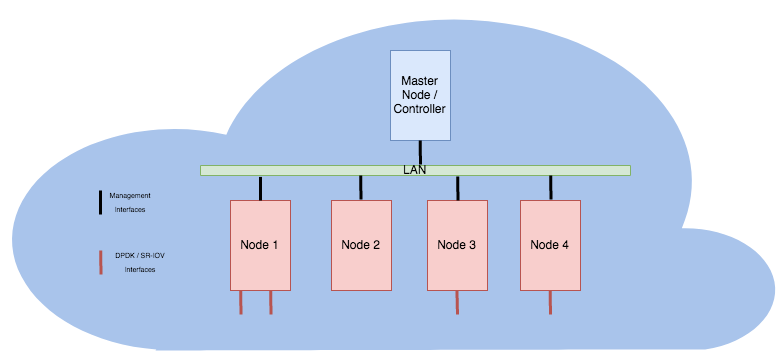
\includegraphics[height=8cm,width=15cm]{pics/ClusterDiag.png}
\end{center}
\caption{A cluster of nodes with one acting as a master. The other nodes can have different hardware features that are supported}
\label{liitekuva}
\end{figure}

The objective of the thesis is to find a fast data plane solution in a container orchestrated environment. There are different scenarios considered based on the availability and features supported by different hosts in the cluster and an intelligent way to deploy the container in the host that meets the latency requirements of the containerized application. To this extend, the topology considers interfaces with DPDK or SR-IOV support that exposed to the external network to some of the hosts in the cluster and also a fast packet forwarding within the cluster to reach the container of interest. In essence, a networking solution that does not affect the flexibility of the cluster and the scheduling decision is done on fly. 

%DPDK utilizes several techniques for better packet processing such as skipping the kernel network stack and running applications on userspace, using poll mode drivers instead interrupt driven ones, hugepages, Direct Memory Access (DMA) and others. Among them, correct utilization of hugepages is an important aspect especially when multiple DPDK based applications are run simultaneously on the same host. Most of the current container run-time applications such as Docker, LXC do not support hugepage isolation and resource limitation. It is possible that one application could end up consuming or pre-allocating all of the available hugepages. Addressing this drawback to support hugepage isolation in containers is another key aspect of this thesis.

Whenever possible, for a better grasp of the performance measurements with DPDK and SR-IOV, a comparative study with and without them is done. For some of the basic tools, only the industry de-facto solutions are considered, such as  Docker for container run-time and Kubernetes for container orchestration. Keeping these constant, the study is on the various networking solutions feasible for them and other aspects described above. The containers used in the experiments run basic DPDK based applications that are shipped with the source code and does a simple forwarding of all packets from one port to another and does not run any application as such. This is a better approach for bench marking latency for a generic scenario.

The next section in the thesis covers the related technologies utilized, their definitions and how they work. This covers the motivation for them and in some cases their evolution. The third chapter covers related work in the field of interest and other miscellaneous information. The forth chapter covers the experiments where various solutions are explored and their latency measurements are bench marked. The fifth chapter puts these measurements together and implements a scheduling algorithm in Kubernetes to pick the best node to meet the latency requirements of the application.

\clearpage
\section{How stuff works}
This section describes the main technologies, tools and other components used in the thesis and how they work.
\subsection{Data Plane Development Kit, DPDK}
DPDK is a "set of libraries and drivers"[1] that enable fast packet processing. It is an open source software framework that can be used to build fast networking applications and is maintained by the Linux Foundation[2]. As compared to a normal kernel network stack, DPDK can provide about twenty five percent [3] improvement in packet processing speed.

The driving factor behind the development of DPDK is to address the handling of extremely fast packet rates, especially in a communication network infrastructure, where the packet sizes are typically smaller and packet rates much higher. The average CPU cycles available for handling a packet is much less. For instance, a 10 Gigabit Ethernet card receiving packets of size 1024 bytes would receive 1.25 million packets per second. A CPU with 2GHz clock cycles handling these packets will have 1600 cycles per packet. For a packet size of 64 bytes, this would be 19.5 million packets per second and 102 cycles per packet. 

DPDK utilizes a verity of techniques to address improve the packet processing. Primarily, it uses Poll Mode Drivers (PMD) instead of interrupt driver drivers to handle packets. In traditional packet handling, when a packet is received, the CPU does a context switching from the userspace process to kernel, runs the Interrupt Service Routine (ISR) and switches back to userspace. This is a big overhead especially for higher packet rates. Poll Mode Drivers run on the userspace and use a dedicated CPU core to handle the traffic on one or multiple interfaces. DPDK uses pthread affinity to disable the kernel scheduler from utilizing those cores.

DPDK utilizes hugepages. Hugepages simply imply bigger page size. The standard Linux page size is 4kB while hugepage size could be 2MB or 1GB. In a normal memory access, the virtual memory address needs to be translated to physical memory before it can be accessed. The critical factor affecting performance is the TLB hit. When bigger page sizes are used, there are fewer pages and higher probability of TLB hit.

Software prefetching in addition to H/W prefetching. 

Intel DDIO : Available only in some supported network cards. Network packets are directly put into L3 cache instead of being DMA'd into main memory.

Cache alignment : Intel cache lines are 64bytes. Cache alignment increases performance. If data fetched from memory is put in different cache lines, it would require multiple cache fetches to retrieve the data. Alignment, putting in one cache line, decreases cache reads.

DPDK uses Direct Memory Access to speed up packet buffer copying. Compared to a normal kernel network
stack, when a packet is received, DPDK uses DMA to directly lift the buffer to user space. In traditional packet handling in the kernel stack involves copying of buffer multiple times such as, from the NIC buffer to kernel socket buffer (skbuf in Linux) and from there to the userspace. This reduces performance due to the copying overhead and also due to loss of localization of data leading to fewer cache hits. The method used in DPDK called zero-copy.

Most of the DPDK components run on the userspace avoiding context switching altogether. The packets received on an interface are DMA'd directly to the poll mode drivers. 

Modes of operation of a DPDK application - Run to completion. Each core is assigned a port or a set of ports. The core does the I/O specifically for that port. It accept the incoming packet, process it and send it out through the same port or set of ports. Pipeline model - One core is dedicated to just I/O. All packets received at this port and then sent to different cores using ring buffers. It is more complex and could result in packet order being not maintained.

%% [1] “DPDK, Data Plane Development Kit”, Retrieved from dpdk.org
%% [2] “Linux Foundation Projects”, Retrieved from https://www.linuxfoundation.org/projects/
%% [3] https://builders.intel.com/university/networkbuilders/course/dpdk-101

The main components of DPDK are the core libraries, Poll Mode Drivers for various supported Network Interface Cards (NICs) and other libraries that deal with packet classification, Quality of Service (QoS) and specific to the different platforms [4]. All of these libraries run on the userpace. Also, apart from theses, DPDK uses PCI drivers in the kernel such as IGB-UIO or VFIO-PCI that do basic functionality. When an interface is bound to DPDK, it is detached from the normal kernel driver and attached to one of these DPDK drivers in the kernel.

%% http://doc.dpdk.org/guides-16.04/prog_guide/overview.html

The core libraries in DPDK has an Environment Abstraction Layer (EAL) which hides or abstracts the platform from the libraries and applications running above it. This also deals with memory allocation in huge pages and PCI related buffer handling. DPDK does not allocate memory at run-time but rather pre-allocates memory during initialization. For packet processing, use memory from pool. Return after use. The libraries related to allocating pool of memory (Mempool) consisting of memory buffer (Mbuf) and lockless queues or ring buffers for handling them are part of the core library.

\subsection{Single Root IO Virtualization, SR-IOV}
SR-IOV is the hardware virtualization of a PCI Express (PCIe) device, or specifically, a NIC, into multiple virtual devices that can be directly assigned to an instance of a virtual machine or a container. SR-IOV has a Physical Function (PF) which acts like a normal PCIe device and multiple Virtual Functions (VF) that act like quite lightweight but with dedicated Rx/Tx queues. In a virtual machine context, the host machine kernel can be bypassed and the packets can flow directly between the VF and PF.

Consider the scenario where one host is running multiple Virtual Machines (VM) and a NIC receiving and transmitting packets for all those VMs. Without any hardware virtualization, when a packet is received by the NIC, it triggers an interrupt to the CPU core that is assigned for handling NIC interrupts. This core services the request and examines the packet. Based on the MAC address or VLAN tag, it forwards the packet to the correct VM by triggering another interrupt on the core that is servicing the virtual machine. This is an overhead since there are multiple interrupt handling in the host even before the packet is transferred to the guest operating system and also there is an extra copy of the packet from the host to the VM. Moreover, when the packet rate is high, one core handling all the packets for all the VMs can be a severe bottle neck for a high packet rate. As an enhancement to this, Intel proposed VMDq [1] technology which has separate packet queues for each core. The received packets are put into one of the queues based on the destination MAC or VLAN. Each core services its packet queue by copying the buffer to the VM. There is distribution of work here and a good performance enhancement. An even further enhancement is SR-IOV in which the NIC has separate packet queues for each Virtual Function. When a packet is received, it is sorted to one of the VF queues based on the destination MAC address or VLAN tag. The VF then pushes the packet up the virtual machine directly without involving the CPU using Direct Memory Access (DMA). SR-IOV needs CPU I/O virtualization technology such as Intel VT-d or AMD-Vi enabled for the DMA to the virtual machine.

%% [1] https://www.intel.com/content/www/us/en/virtualization/vmdq-technology-paper.html
\subsection{Container}
A container is an isolated execution environment which includes any necessary run time dependencies and libraries needed for the application that it packages. It could be thought of as a software that runs on the host with its own slice of the system resources such as network, file systems, user groups, etc. but isolated from other processes. Containers are built on namespaces and control groups which are a part of the Linux kernel.

As per Linux man pages, namespace is an abstraction layer on "global system resources" that provides isolated instance of the resource to the processes that are members of the namespace. Linux provides six different namespaces, Inter Process Communication (IPC) including POSIX and System V message queues, Network, Mount, Process Identifier (PID), User and UTS [1]. With network namespace, the processes in the new namespace can add new network devices without them being available to host network namespace and vice versa. Similarly, with mount namespace, different file systems can be mounted and processes within this namespace cannot access host file system. Namespaces can be created using Linux system call unshare. The context of namespaces that every process belongs to stored in a sub-folder under proc file system as shown below.
%% [1] Linux man paages; man 7 namespaces; man unshare
\begin{lstlisting}[basicstyle={\small\ttfamily}]
$ ls -l /proc/$$/ns | awk '{print $1"\t"$(NF-2)$(NF-1)$NF}'
lrwxrwxrwx      cgroup->cgroup:[4026531835]
lrwxrwxrwx      ipc->ipc:[4026531839]
lrwxrwxrwx      mnt->mnt:[4026531840]
lrwxrwxrwx      net->net:[4026532009]
lrwxrwxrwx      pid->pid:[4026531836]
lrwxrwxrwx      pid_for_children->pid:[4026531836]
lrwxrwxrwx      user->user:[4026531837]
lrwxrwxrwx      uts->uts:[4026531838]

\end{lstlisting}

Below is an example of using namespaces to create an isolated environment. The current process id in a bash shell can be found out using "\$\$". Then use unshare command to create a new namespace. Here the arguments "pid" and "net" signifies new namespaces for process ids and network. The argument "mount-proc" tells the command to mount the proc file system. The "fork" option makes a fork of the current process before creating the namespace and attaching the child process to it. 

\begin{lstlisting}[basicstyle={\small\ttfamily}]
$ echo $$ 
8009
$ unshare --fork --pid --net --mount-proc bash
root:~# ip l
1: lo: <LOOPBACK> mtu 65536 qdisc noop state DOWN mode DEFAULT group
    default qlen 1000 link/loopback 00:00:00:00:00:00
    brd 00:00:00:00:00:00
root:~# ps -aef
UID        PID  PPID  C STIME TTY          TIME CMD
root         1     0  0 13:37 pts/26   00:00:00 bash
root        12     0  0 13:44 pts/30   00:00:00 -bash
root        32     1  0 13:52 pts/26   00:00:00 ps -aef
root:~#                                  

$ ps -aef | grep bash | grep root | awk '{print $1"\t"$2"\t"$3"\t"$8}'
root     31215  8009    sudo
root     31294 31215    sudo
root     31295 31294    unshare
root     31296 31295    bash

$ nsenter -m -u -i -n -p  -t 31296
root:/# ps -aef
UID        PID  PPID  C STIME TTY          TIME CMD
root         1     0  0 13:37 pts/26   00:00:00 bash
root        12     0  0 13:44 pts/30   00:00:00 -bash
root        30    12  0 13:45 pts/30   00:00:00 ps -aef
root:/# 

\end{lstlisting}

\texttt{Add a network bridge within the new namespace and check outside.}

\begin{lstlisting}[basicstyle={\small\ttfamily}]
root:~# brctl addbr asd
root:~# ip l
1: lo: <LOOPBACK> mtu 65536 qdisc noop state DOWN mode DEFAULT group
    default qlen 1000 link/loopback 00:00:00:00:00:00
    brd 00:00:00:00:00:00
2: asd: <BROADCAST,MULTICAST> mtu 1500 qdisc noop state DOWN mode
    DEFAULT group default qlen 1000 link/ether 4a:18:f1:3c:9c:b2
    brd ff:ff:ff:ff:ff:ff
\end{lstlisting}

Control groups on the other hand are useful in limiting the resource consumption. Control groups or cgroups are organized hierarchically. 

Any description of containers is incomplete without a comparison to virtual machines. A virtual machine emulates an entire machine. There is a hypervisor that runs on the host machine that emulates the underlying hardware. Then a complete operating system running on top of it. The advantage of virtual machine is that it is completely isolated from the host machine. The run environment can be guaranteed in spite of the host hardware and operating system. While at the same time, virtual machines can be heavy weight and resource consuming. In contrast, the container essentially runs completely on the host. It uses namespaces and control groups for isolation of the container from the host. As a result, they are much more easy to boot up, lightweight and picking up in popularity when compared to virtual machines [].

%% []

is the easy replication of the development environment in scenarios such as in deployment. Containers have become de-facto standard for application packaging/deployment and there is a need to explore fast data processing solutions in a containerized environment.

\subsubsection{Container Networking Interface}
Container Networking Interface is a proposal for 
%% https://github.com/containernetworking/cni/blob/master/SPEC.md

\subsection{Kubernetes}
Kubernetes is an open source orchestration system that manages containerized applications. It can be used for 

k8s architecture (Chapter 4)
One master and many workers. "Cluster is driven using API calls to controllers" Architecture diagram (https://kubernetes.io/docs/concepts/architecture/cloud-controller/)

Components : Master, worker nodes and Controllers, Services, Pods, Namespaces, Network and Storage

k8s master has Kube API server, kube-scheduler and etcd database.
Also a cloud controller manager, other 3rd party softwares, DNS, etc. All needed for a production cluster. Kube API server updates etcd. Only this interacts with etcd.
Kube api server acts like an access point to both "internal and external traffic" and "master process to the entire cluster".
Scheduler decides which node to deploy the pod. Decision is  based on an algorithm. User defined algo could be used or the original one modified. Intel node discovery feature could be used with scheduler to figure out where to deploy.

---- No more detailed writing
k8s worker has kublet and kube-proxy
Kubelet for local configurations

\clearpage
\section{Related work and Misc}
1. Related work in the field
2. Experimental runs, how many and what is measured
3. Considerations - Packet generators


\clearpage
\section{Core - Implementation, experiments}
This section covers the actual experimentation part of the thesis with the motivation to do so. The first two subsections explore a fast data path in container running in a single host. The first of those is a DPDK based container running on a host with SR-IOV interfaces being used for forwarding packets from the NIC to the container and back. The second subsection is a study on Open vSwitch (OvS) and DPDK acceleration. In this case, there is a OvS bridge receiving packets from the NIC and forwarding to the container and back. There is a comparative study to understand how much acceleration is brought about by DPDK.

The remaining subsections consider only a cluster environment with Kubernetes. For a fast data path in this case, multiple scenarios have been considered and some potential solutions discussed and experimented with. For this, initially a Kubernetes cluster is built on bare metal using MAAS (Metal-as-a-Service) and \lstinline{kubeadm} or Juju. Then the different scenarios are outlined and discussed one after the other in a detailed manner.

\subsection{Container on DPDK and SR-IOV}
A default docker container built on a bare Ubuntu image creates by default one interface that is connected to "docker0" bridge on the host. This is the default networking option in Docker []. 
%% https://docs.docker.com/network/#scope-of-this-topic

\begin{lstlisting}[basicstyle={\small\ttfamily}]
$ docker run -it ubuntu:latest /bin/bash
root@f8344e977497:/# ip l
bash: ip: command not found
root@f8344e977497:/# ifconfig 
eth0: flags=4163<UP,BROADCAST,RUNNING,MULTICAST>  mtu 1500
        inet 172.17.0.2  netmask 255.255.0.0  broadcast 172.17.255.255
        ether 02:42:ac:11:00:02  txqueuelen 0  (Ethernet)
        RX packets 25  bytes 4140 (4.1 KB)
        RX errors 0  dropped 0  overruns 0  frame 0
        TX packets 0  bytes 0 (0.0 B)
        TX errors 0  dropped 0 overruns 0  carrier 0  collisions 0

lo: flags=73<UP,LOOPBACK,RUNNING>  mtu 65536
        inet 127.0.0.1  netmask 255.0.0.0
        loop  txqueuelen 1000  (Local Loopback)
        RX packets 0  bytes 0 (0.0 B)
        RX errors 0  dropped 0  overruns 0  frame 0
        TX packets 0  bytes 0 (0.0 B)
        TX errors 0  dropped 0 overruns 0  carrier 0  collisions 0
\end{lstlisting}
The host docker0 bridge in the same sub-net
\begin{lstlisting}[basicstyle={\small\ttfamily}]
$ ip a | grep -A 3 docker0
7: docker0: <NO-CARRIER,BROADCAST,MULTICAST,UP> mtu 1500 qdisc noqueue state DOWN group default 
    link/ether 02:42:29:09:76:49 brd ff:ff:ff:ff:ff:ff
    inet 172.17.0.1/16 brd 172.17.255.255 scope global docker0
       valid_lft forever preferred_lft forever
    inet6 fe80::42:29ff:fe09:7649/64 scope link 
       valid_lft forever preferred_lft forever
\end{lstlisting}

Docker supports other networking options such as host, overlay, macvlan. Host networking option in Docker removes the network isolation between the host and the container. Overlay is an overlay network and can be used to connect to other containers in different host managed by Docker swarm. Macvlan assigns a MAC address to the virtual interface in the container and exposes it to a parent host physical interface making it look like a real physical interface. All of the above options are suited for specific use cases. The final option in Docker networking, using network plugins, is the most interesting one. It is an interface to use third part networking plugins, or CNI plugins. The open source CNI plugins for SR-IOV and DPDK could be used to explore fast data path networking in containers.

The test setup consists of two physical machines. Both the machines have a management interface and two SR-IOV interfaces each. The SR-IOV interfaces are connected in back to back forming a closed loop as show in the figure below.
\begin{figure}[htb]
\begin{center}
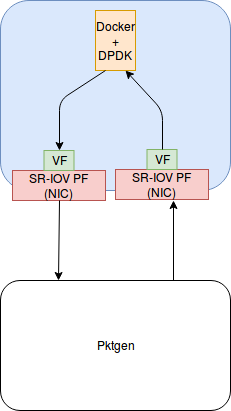
\includegraphics[height=8cm]{pics/ContainerOnDPDKandSRIOV.png}
\end{center}
\caption{Test topology. DPDK based pktgen on one side and a Docker container with DPDK and SR-IOV on the other.}
\label{liitekuva}
\end{figure}

One of the machines is used as a packet generator while the other one utilizes virtualization of SR-IOV to push the packet directly to the container. The container also runs a DPDK application that just forwards the packets received on one port to the other. To run DPDK based application, enable SR-IOV Virtual Functions and use CNI plugins with Docker, the host environment has to be configured as described below.

For running DPDK based applications, hugepages should be enabled in the host machine. The hugepage sizes that supported in the most common Linux distributions are 2MB and 1GB. If 1GB hugepages are to be used, it is recommended to have them configured at boot time by setting some Kernel boot parameters. This it to ensure the availability of such a large contiguous memory, 1GB, in main memory. This is mostly not possible at run time due to fragmentation. The kernel boot parameters could be set by editing \lstinline{/etc/default/grub} and updating GRUB with \lstinline{update-grub} command. For instance, edit \lstinline{GRUB_CMDLINE_LINUX} to include, \lstinline{GRUB_CMDLINE_LINUX="default_hugepagesz=1G hugepagesz=1G hugepages=4"}. Now update GRUB, reboot machine and check boot parameters and consequently hugepage availability as follows,

\begin{lstlisting}[basicstyle={\small\ttfamily}]
$ cat /proc/cmdline 
BOOT_IMAGE=/boot/vmlinuz-4.4.0-131-generic default_hugepagesz=1G hugepagesz=1G hugepages=4
$ cat /proc/meminfo | grep -i hugepages_
HugePages_Total:       4
HugePages_Free:        4
HugePages_Rsvd:        0
HugePages_Surp:        0
Hugepagesize:    1048576 kB
\end{lstlisting}

The hugepages have to be mounted on the host. In some versions of Linux distributions, for instance, in Ubuntu 16.04 and higher, they are mounted automatically in \lstinline{/dev/hugepages}. It is also possible to isolate the CPU cores that will be used for the DPDK application using boot paramters so that the Kernel scheduler does not use them. For instance, \lstinline{GRUB_CMDLINE_LINUX="default_hugepagesz=1G hugepagesz=1G hugepages=4 isolcpus=2,3,4,5,6,7"}

DPDK supports different Linux Kernel drivers such as UIO, VFIO, etc. []. VFIO is used in most of the cases in the thesis since, as stated in DPDK documentation, it is "more robust and secure" []. VFIO kernel module if supported, is shipped with the OS. It also needs IO virtualization such as Intel VT-d and that needs to be enabled in BIOS. IOMMU has to be set as a Kerenel boot parameter,
\begin{lstlisting}[basicstyle={\small\ttfamily}]
$ cat /proc/cmdline 
BOOT_IMAGE=/boot/vmlinuz-4.4.0-131-generic default_hugepagesz=1G hugepagesz=1G hugepages=4 intel_iommu=on
\end{lstlisting}

Setting up a SR-IOV interface for virtualization requires IOMMU and Intel VT-d support which are also needed when using VFIO driver as noted above. The number of VFs to be enabled can be set using \lstinline{sys} virtual file system in 
\lstinline{/sys/class/net/$IFNAME/device/sriov_numvfs} where \lstinline{$IFNAME} is the name of the SR-IOV interface as displayed in \lstinline{ip link} command. MAC address needs to be specifically set for each VF using \lstinline{ip link set dev $IFNAME vf $i mac aa:bb:cc:dd:ee:01} where \lstinline{$i} is the VF count. The Physical Function uses this to forward a received packet to the correct VF and hence directly to the container or VM it is exposed to.

For using third party CNI plugins, when a Docker container is spawned, it looks for network configuration file in the default location, lstinline{/etc/cni/net.d/} and binary of the plugin in lstinline{/opt/cni/bin/}. The plugin used for this test case is SR-IOV CNI plugin with support for DPDK []
%% https://github.com/intel/sriov-cni

The topology needs a DPDK based container on one side and a packet generator on the other. For building a container that can run a DPDK application, the idea is to start with a base image of some standard Linux distribution such as Ubuntu 16.04, install the required libraries, tools including some debugging tools such as GNU debugger (GDB). DPDK compilation would require Linux header files and other standard build tools, make, etc. Then fetch the DPDK code, compile the libraries and the required application, testpmd. Some extra compile time flags are used to enable debugging with GDB.

\begin{lstlisting}[basicstyle={\small\ttfamily}]
$ git clone http://dpdk.org/git/dpdk dpdk

$ cat > build-dpdk.sh<<EOF
echo "Build DPDK"
make install T="\$RTE_TARGET" EXTRA_CFLAGS="-g -O0" -j8
if [ \$? != 0 ]; then
    echo -e "\tBuilding DPDK failed"
    exit 1
fi
cd app/test-pmd/
make -j8
EOF

$ chmod +x build-dpdk.sh
$ cat > Dockerfile <<EOF
FROM ubuntu:16.04
RUN apt-get update; apt-get install -y apt-utils build-essential less make kmod vim pciutils libnuma-dev python gdb linux-headers-$(uname -r);
COPY ./dpdk /root/dpdk
COPY ./build-dpdk.sh /root/dpdk/build-dpdk.sh
WORKDIR /root/dpdk/
ENV RTE_SDK "/root/dpdk"
ENV RTE_TARGET "x86_64-native-linuxapp-gcc"
RUN ./build-dpdk.sh
EOF

$ docker build -t dpdk-docker:latest .
\end{lstlisting}

Now, as is visible from Fig.[], one VF per SR-IOV interface is sufficient for this experiment. However, one VF from each SR-IOV interface is exposed to the container. The CNI plugin configuration used is as follows,
\begin{lstlisting}[basicstyle={\small\ttfamily}]
$ cat /etc/cni/net.d/10-sriov-dpdk.conf
{
    "name": "net1",
    "type": "sriov",
    "if0": "enp1s0f1",
    "if0name": "if0",
    "dpdk": {
        "kernel_driver":"ixgbevf",
        "dpdk_driver":"igb_uio",
        "dpdk_tool":"\$RTE_SDK/usertools/dpdk-devbind.py"
    }
}
\end{lstlisting}

In the configuration above, \lstinline{type} is always \lstinline{sriov} for this plugin, \lstinline{if0} is the name of the SR-IOV interface or PF, \lstinline{if0name} is the name inside the container and within dpdk parameters, \lstinline{kernel_driver} is the current Kernel driver the interface is using, \lstinline{dpdk_driver} is the DPDK driver that needs to be used, such as VFIO and \lstinline{dpdk_tool} is a tool that is shipped with DPDK source code that can be used to binding interfaces to DPDK. The above configuration could be replicated with different \lstinline{if0} and \lstinline{if0name} for the VF from second SR-IOV interface.
%% [] https://github.com/intel/sriov-cni

To run DPDK application in the container, the container has to be run in privileged mode so that it bind the interfaces, get hugepage information, etc. This can be done with the \lstinline{--privileged} flag in Docker. Also, the hugepage mount location has to be mounted in the container as a volumn. Docker run command is as follows,
\begin{lstlisting}[basicstyle={\small\ttfamily}]
docker run -it -v /dev/hugepages:/dev/hugepages --privileged dpdk-docker:gdb /bin/bash
\end{lstlisting}

Inside the container, start testpmd application and configure it for forwarding packets received on one port to the other. If there are an even number of ports attached to DPDK, this is also the default behavior. This can be checked with \lstinline{show config fwd} command inside testpmd. Start Rx/Tx with \lstinline{start} command.

\begin{lstlisting}[basicstyle={\small\ttfamily}]
testpmd> show config fwd
io packet forwarding - ports=2 - cores=1 - streams=2 - NUMA support enabled, MP over anonymous pages disabled
Logical Core 1 (socket 0) forwards packets on 2 streams:
  RX P=0/Q=0 (socket 0) -> TX P=1/Q=0 (socket 0) peer=02:00:00:00:00:01
  RX P=1/Q=0 (socket 0) -> TX P=0/Q=0 (socket 0) peer=02:00:00:00:00:00

testpmd> start
\end{lstlisting}

On the packet generator side, DPDK based packet generator "pktgen" is used. Since this is a DPDK application, similar steps as above are repeated. Bind both interfaces to DPDK and start pktgen.
Latency has to be specifically enabled in DPDK interfaces in pktgen and the packet size set to 96 so that there is room in the buffer for time stamping. Here, we set the destination MAC address as the MAC address of the receiving VF, otherwise the packets get dropped at PF.

\begin{lstlisting}[basicstyle={\small\ttfamily}]
./app/x86_64-native-linuxapp-gcc/pktgen -l 0-3 -n 4 --proc-type auto --log-level 7 --socket-mem 2048 --file-prefix pg -- -T -P --crc-strip -m [1:2].0 -m [2:3].1 -f themes/black-yellow.theme
pktgen> enable 1 latency
pktgen> set 1 dst mac aa:bb:cc:dd:ee:00
pktgen> set 1 size 96
pktgen> start 1
\end{lstlisting}
Above, 1 refers to the port number we are generating packets. And with \lstinline{start 1}, packets are generated at approximately 11 million packets per second (Mpps), as reported by pktgen.

The latency was about 800 micro seconds.

For a comparative study, instead of the host with DPDK based container and packet forwarded through a DPDK based application (testpmd), let the packet packet processing happen via. the standard Linux kernel stack. For this, create a Linux bridge and add the two interfaces to it.

The latency was about 8700 micro seconds for a packet rate of 10Mpps.

\subsection{Container on OVS-DPDK}
The test setup in the previous section used was probably the simplest network possible. The machines were directly connected and the traffic blindly forwarded from one port to another. In a more realistic scenario, there could be multiple containers running on the host and packets forwarded between them. In a container orchestrated environment with Kubernetes, these containers or pods could very well reside in different hosts. This calls for exploring a more generic networking solution.

The default networking provided with Docker, using \lstinline{docker0} bridge is a good solution that would work for containers in one host. Similarly, the overlay network driver in Docker and other third part network plugins such as using Flannel[], Weave Net[2], Calico[3], etc. which also work with Kubernetes are also solutions that could work with little hassle. But none of these methods provide support for a fast data path using DPDK or support virtualization with SR-IOV VFs. However, Open vSwitch is one plausible solution. It supports DPDK and provides a way to easily configure the network using Open Flow. Though it might be an overhead in a simple topology, it could scale well when the network is more complicated with multiple hosts and different types of interfaces such as for management and data since it also supports setting up tunneling interfaces to configure an overlay network which could be helpful with Kubernetes. However, whether the overlay network can support a DPDK based fast data path is still to be explored.
%% [1] https://github.com/coreos/flannel
%% [2] https://github.com/weaveworks/weave
%% [3] https://docs.projectcalico.org/v2.0/getting-started/kubernetes/

This section uses OvS with DPDK and a container with DPDK application, testpmd on one side. Both the SR-IOV interfaces are this time connected to the OvS bridge. The other packet generator side is unchanged as the previous test scenario.

OvS releases page[1] notes the compatible versions of DPDK with OvS and also the compatible version of OvS for different Linux Kernel versions. In this experiment, the Linux Kernel version used is \lstinline{4.4.0-131-generic}. Correspondingly, the latest compatible version of OvS is 2.9.x and DPDK version compatible this version of OvS is 17.11.3
%% [1] http://docs.openvswitch.org/en/latest/faq/releases/

To use Open vSwitch (OvS) with DPDK data path, DPDK needs to be built as in normal scenario but with the correct version as described above. The environment variables \lstinline{RTE_SDK} and \lstinline{RTE_TARGET} should be set. The former is the path to DPDK source code and the later is the build target environment, or \lstinline{x86_64-native-linuxapp-gcc} in this case. The OvS needs to be configured with \lstinline{--with-dpdk="$RTE_SDK/$RTE_TARGET"} and compiled.

DPDK parameters such as lcore, memory and other typical settings used with most other DPDK applications can be set in the OvS data base as shown below,

\begin{lstlisting}[basicstyle={\small\ttfamily}]
sudo ovs-vsctl --no-wait set Open_vSwitch . other_config:dpdk-init=true
sudo ovs-vsctl --no-wait set Open_vSwitch . other_config:dpdk-lcore-mask=0x0F
sudo ovs-vsctl --no-wait set Open_vSwitch . other_config:dpdk-socket-mem=256
sudo ovs-vsctl --no-wait set Open_vSwitch . external-ids:system-id="${HOSTNAME}id"
\end{lstlisting}

The system ID could come in handy when setting up an overlay network with OvS. Most other steps in setting up OvS with DPDK are quite straighforward or well documented and not listed here.

The final part of the previous section had a Linux bridge with interfaces attached to it and packets forwarded as a normal bridge would do, flood. In this test, something similar in theory is done with an OvS bridge. But, the interfaces are bound to DPDK and then attached to an OvS bridge. Also couple of flows are added to the bridge to forward the packets received on one interface to the other and vice versa instead of flooding. The commands are shown in detail below.

\begin{lstlisting}[basicstyle={\small\ttfamily}]
$ ovs-vsctl add-br dpdk-br -- set bridge dpdk-br datapath_type=netdev
$ ovs-vsctl add-port dpdk-br p1 -- set Interface p1 type=dpdk options:dpdk-devargs=0000:01:00.0 ofport_request=1
$ ovs-vsctl add-port dpdk-br p2 -- set Interface p2 type=dpdk options:dpdk-devargs=0000:01:00.1 ofport_request=2
$ ovs-ofctl add-flow ext1 in_port=2,action=output:1
$ ovs-ofctl add-flow ext1 in_port=1,action=output:2
\end{lstlisting}

Now from the other end, packets were generated at an average of 10Mpps and the latency was observed to be around 800 micro seconds. This is the same value of latency observed in the previous section with SR-IOV VF exposed to a container and a DPDK based application running on a container. This shows that OvS running as a DPDK application does not add any additional latency. Also, counter intuitively, a container running DPDK application gives same latency as OvS on DPDK. This implies, a container as such does not add any latency to slow down the processing of packets. Which it should not theoretically as well.

Now, the next logical step is to add a container in between the two interfaces and forward the packets to a DPDK application, testpmd, running inside the container and forward the packets back to the packet generator. To expose DPDK interfaces to a container via. OvS, OvS uses \lstinline{vhostuser} port on the host side. This creates a UNIX domain socket which needs to be exposed to the container. In DPDK application, a \lstinline{virtiouser} port is created using this socket file. Now, flows are added to forward packets between the DPDK interface and \lstinline{vhostuser} ports. The packets received at \lstinline{vhostuser} will be picked by \lstinline{virtiouser} and thus the DPDK application.

\begin{lstlisting}[basicstyle={\small\ttfamily}]
$ ovs-vsctl add-port dpdk-br vhu-p1 -- set Interface vhu-p0 type=dpdkvhostuser
$ ovs-vsctl add-port dpdk-br vhu-p2 -- set Interface vhu-p1 type=dpdkvhostuser
$ ovs-ofctl add-flow dpdk-br in_port=1,actions=output:3
$ ovs-ofctl add-flow dpdk-br in_port=4,actions=output:2
\end{lstlisting}

The port numbers in OvS could be verified with command \lstinline{ovs-ofctl dump-ports-desc dpdk-br}. The UNIX domain sockets are created by default in location \lstinline{/usr/local/var/run/openvswitch/}. So, this also has to be mounted while running DPDK Docker apart from the hugepages mount.

\begin{lstlisting}[basicstyle={\small\ttfamily}]
docker run --privileged -it -v /dev/hugepages:/dev/hugepages -v /usr/local/var/run/openvswitch:/var/run dpdk-docker:gdb /bin/bash
\end{lstlisting}

While running the DPDK application inside container, the PCI devices are disabled so that the application does not look for physical ports and virtual devices are created using the two \lstinline{virtiouser} ports.

\begin{lstlisting}[basicstyle={\small\ttfamily}]
./testpmd -c 0xf -n 4 -m 1024 --no-pci --vdev=virtio_user0,path=/var/run/vhu-p1 --vdev=virtio_user1,path=/var/run/vhu-p2 --file-prefix=container -- -i
\end{lstlisting}

Now, as before, the other host starts sending packets at 11Mpps and the latency was observed to be approximately 5000 micro seconds.

\subsection{Fast packet processing in Kubernetes}
The previous two sections dealt with the networking aspects when containers were hosted on just one  host and packets were generated from another. But in a real scenario, there would be a cluster of many hosts with some container orchestration such as Kubernetes managing them. When a request to deploy a new container or rather a pod, in Kubernetes is received, Kubernetes decides on which host to deploy depending on the requirements to run the pod such as available memory, CPU cores and any other constraints that may be provided. Kubernetes has to find a host that fits all the bills. The networking aspects in such a scenario could get tricky. In a Kubernetes deployed pod, there has to be one management interface to communicate with kubelet, which runs on all the worker nodes. Then, for fast packet processing, some other pod interfaces that are connected to the DPDK bound physical interfaces. These DPDK interfaces could be exposed to the external network.

Now, when a pod is being deployed in Kubernetes and if it needs external DPDK interfaces, Kubernetes has to decide on which host to deploy the pod. There are three scenarios to be considered here.

The first scenario is when the required number of external DPDK interfaces for the pod is present in all of the Kubernetes worker nodes. In this case the pod could be deployed in any of the hosts and this does not become a constraint. The only question to be answered here is how to expose multiple interfaces to a pod. Kubernetes in its default state supports only one interface.

The second scenario is when the required external DPDK interaces for the pod are present in just some of the worker nodes. In this case, the Kubernetes scheduler, which runs on the master, needs some mechanism to find out which hosts satisfy this criteria.

The third scenario is the trickiest. If the required number of DPDK interfaces are say, three, and there are three worker nodes with one DPDK interface each. Here, the decision on which host to deploy the pod cannot be made based on meeting this criteria but rather, there has to be some fast data path between the worker nodes. Earlier it was noted that every Kubernetes pod has a default management interface which is used to communicate with the kubelet running on the worker node. This also implies, there is a management interface on each worker node that is reachable to each other and also the master. This is also one of Kubernetes networking requirements[].
%% [] https://kubernetes.io/docs/concepts/architecture/master-node-communication/

The above three scenarios and their potential solutions are discussed in the next few sections. But first let's build a Kubernetes cluster.

\subsection{Building a Kubernetes cluster}
The Kubernets cluster is built from bare metal machines. To build a cluster from these hosts, MAAS or Metal as a Service, is used. MAAS is open source software developed by Canonical[]. MAAS needs a central machine which is the controller. The controller runs a DHCP server. Other nodes to be added to the cluster should be placed in the sub-net and configured to boot from network or PXE boot. The controller was configured to use Ubuntu 16.04 images for commissioning the nodes. The topology of the machines is show in Figure 1. 
%% [] https://www.canonical.com/

\begin{figure}[htb]
\begin{center}
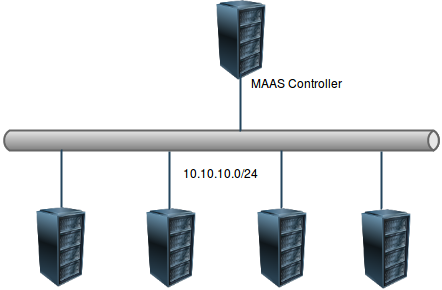
\includegraphics[height=8cm]{pics/MAAS-topology.png}
\end{center}
\caption{Topology of cluster built with MAAS}
\label{liitekuva}
\end{figure}

A MAAS cluster can have two types of controllers, region and rack controller. Since, the setup being built is quite small and the machines can be physically attached to a subnet using only a bridge, just one controller is used. It acts both as region and rack controller. Adding nodes to the cluster can be done by attaching the new machine to the subnet and setting the interface to PXE boot. The controller sends the boot image through the local area network and runs some cloud init scripts to set up the new machine. The new machine goes into "Ready" state and can be acquired while deploying some application such as Kubernetes. Functioning quite like a cloud. For the nodes to have external connectivity, the controller's IP tables have to be modified to enable NAT.

To deploy Kubernetes, the easiest approach, as documented in[], is to deploy it with Juju. This essentially, deploys a out-of-box Kubernetes with one or more masters, worker nodes and other applications such as etcd, flannel, easyrsa, etc. "etcd" is used to distributed key value storage, "flannel" is the network plugin and "easyrsa" is for generating certificates for TLS. For this approach, Juju needs to be deployed first and it needs a dedicated controller. One way is to start a virtual machine in MAAS controller and add it to the cluster and use it as Juju controller. Another approach would be to use any other node in cluster for this. The choice depends on how machines are available and how many are needed for Kuberentes since Juju controller cannot be in Kubernetes. In this experiment, the virtual machine method was used. Juju was then used to deploy a minimal Kubernetes cluster with two machines using the command, \lstinline{juju deploy cs:bundle/kubernetes-core-251}.

To deploy a simple pod in Kubernetes, create pod manifest file and use \lstinline{kubectl} commands to create the pod.

\begin{lstlisting}[basicstyle={\small\ttfamily}]
$ cat > helloworld.yaml <<EOF
apiVersion: v1
kind: Pod
metadata:
  name: test-pod
spec:
  containers:
  - name: test-container
    image: ubuntu:latest
    command: ["/bin/bash"]
    args: ["-c", "echo SUCCESS; while true; do sleep 1; done"]
EOF
$ kubectl create -f helloworld.yaml
$ kubectl get pods
NAME            READY     STATUS        RESTARTS   AGE
test-pod        1/1       Running       0          5s
$ kubectl logs test-pod
SUCCESS
\end{lstlisting}

Another way to deploy Kubernetes is using the tool \lstinline{kubeadm}. This is a Kubernetes project that is still in beta stage but quite good for development purposes. The deployment of Kubernets is quite bare minimalistic while comapred to deploying with Juju. This gives a bit more control. With \lstinline{kubeadm}, the network has to be installed separately which is ideal for most of the work in the thesis since, it can be easily tweaked and modified.


\subsection{Scenario 1, Multus}
\subsection{Scenario 2, Node feature discovery}
Kubernetes incubator project - Node Feature Discovery
\subsection{Scenario 3, Kubernetes with OvN}
Exposing external interface and routing within

%% http://docs.openvswitch.org/en/latest/howto/userspace-tunneling/

\clearpage
\section{Kubernetes scheduler to pick the right node}



\clearpage
\section{Results and Conclusions}

\clearpage
\thesisbibliography
\begin{thebibliography}{99}

\bibitem{container-vm-comparison} Joy,\ M.,\ A., Performance Comparison Between Linux Containers and Virtual Machines. \textit{International Conference on Advances in Computer Engineering and Applications.} IMS Engineering College, Ghaziabad, India, 2015
\end{thebibliography}

%% Appendices
%% If you don't have appendices, remove \clearpage and \thesisappendix below.
\clearpage
\thesisappendix
\section{Appendix A\label{LiiteA}}

\end{document}